\documentclass[a4paper]{scrartcl}
\usepackage[utf8]{inputenc}
\usepackage{ngerman}
\usepackage{mathtools}
\usepackage{amssymb}
\usepackage{pdfpages}
\usepackage{mathtools}
\usepackage{listings}
\usepackage{tikz}
\usepackage{qtree}
\usepackage{hyperref}

\title{Scriptum Grundlagen der Informatik}
\date{WS 2013/2014}
\author{Markus Klemm.net}

\lstdefinestyle{customc}{
  belowcaptionskip=1\baselineskip,
  breaklines=true,
  frame=L,
  xleftmargin=\parindent,
  language=C,
  showstringspaces=false,
  basicstyle=\footnotesize\ttfamily,
  keywordstyle=\bfseries\color{green!40!black},
  commentstyle=\itshape\color{purple!40!black},
  identifierstyle=\color{blue},
  stringstyle=\color{orange},
}

\begin{document}
\maketitle
\tableofcontents

\section{Aussagenlogik}

\paragraph{Ziel}
Aussagen formulieren die entweder wahr oder falsch sind. Eine atomare Aussage ist eine Aussage, die sich nicht in kleinere Bestandteile zerlegen lässt, z.B.: es regnet oder die Straße ist nass. Mit logischen Verknüpfungen lassen sich daraus neue Aussagen erzeugen.

Jede atomare Aussage ist eine Formel der Aussagenlogik. Diese heißen Atomformeln. Atomformeln bezeichnen wir mit Kleinbuchstaben oder Wörtern in Kleinbuchstaben.

Wenn F,G Formeln der Aussagenlogik sind, dann auch $(F \wedge G), (F \vee G), (\neg F).$

Um Klammern zu sparen, legen wir folgende Prioritäten fest:

\begin{tabular}{c|c}

Operator & Priorität \\ \hline
$\neg$ & höchste \\
$\wedge \vee$ & \\
$\Rightarrow \leftrightarrow$ & \\
$\equiv$ & Niedrigste \\
\end{tabular}

Bsp: Formeln der Aussagenlogik sind : regnet, nass, $ x, y, x \wedge  y, \neg X, x \vee y $. Keine Formeln der Aussagenlogik: $\wedge x , x \wedge \vee y $

\subsection{Semantik}
\paragraph{Definition}
Eine Belegung einer Formel F der Aussagenlogik ist eine Zuordnung von Wahrheitswerten wahr (1) oder falsch (0). Zu den Atomformeln in F. Daraus ergibt sich der Wahrheitswert einer Formel der induktiv definiert ist:
\subparagraph{}
Eine Atomformel ist wahr genau dann, wenn sie mit wahr belegt ist.
\subparagraph{}
Die Formel $F \wedge G$ ist wahr genau dann, wenn F wahr und G wahr sind.
Die Formel $F \vee G$ ist wahr genau dann, wenn F wahr oder G wahr sind.
Die Formel $\neg F$ ist wahr genau dann, wenn F falsch ist.
Die Formel 

\begin{tabular}{c|c|c|c|c|c|c}

F & G & $F \wedge G$ &$ F \vee G$&$\neg F$ & $F \Rightarrow G$ & $F \leftrightarrow G$ \\ \hline
0&0&0&0&1&1&1 \\
0&1&0&1&1&1&0 \\
1&0&0&1&0&0&0 \\
1&1&1&1&0 &1&1\\

\end{tabular}

Bsp: Wenn regnet eine Atomformel mit der Bedeutung "`es regnet ist"' und nass eine Atomformel mit der Bedeutung "`die Straße ist nass"', dann bedeutet $regnet \wedge nass$  "`es regnet und die Straße ist nass"'.
Wenn regnet, nass mit wahr belegt werden, ist auch $regnet \wedge nass$ wahr.
\subparagraph{}
Definition: Die Operatoren $\Rightarrow$ (Implikation) und $\leftrightarrow$ (Äquivalenz) sind definiert durch

\[F \Rightarrow G = \neg F \vee G\]
\[F \leftrightarrow G = ( F \Rightarrow G ) \wedge ( G \Rightarrow F)\]

Bsp: Der Beitrag y einer Zahl x lässt sich berechnen durch

\begin{lstlisting}[numbers=left, tabsize=4, style=customc]
if (x>=0)
{
	y=x
}
else
{
	y=-x
}
\end{lstlisting}

Die Wirkung dieser Anweisung lässt sich beschreiben durch die Formel
\[(x\geq 0 \Rightarrow y = x) \wedge (\neg (x\geq 0)\Rightarrow y=-x)\]

\paragraph{Definition}
Eine Formel F heißt Tantologie, wenn F unter jeder Belegung wahr ist. Mit dem Symbol T bezeichnen wir eine Tantologie.
Mit $\perp$ bezeichnen wir eine Formel die unter jeder Belegung falsch ist. (unerfüllbar)
\paragraph{Definition}
Wir schreiben F=G, wenn F,G unter jeder Belegung die gleichen Wahrheitswerte besitzen.
\paragraph{Rechenregeln}
\[F\vee (G\wedge H)= (F\vee G)\wedge(F\vee H)\]
\[F\wedge (G\vee H) = (F\wedge G)\vee (F\wedge H)\]
\[\neg (F\vee G) = \neg F \wedge \neg G\]
\[\neg (F \wedge G) = \neg F \vee \neg G\]
\[\neg \neg F = F\]

\subparagraph{Beispiel} (logische Kontraposition)\\
$F \Rightarrow G = \neg F \vee G = \neg \neg G \vee \neg F = \neg G \Rightarrow \neg F$

\subparagraph{Definition}
Wir schreiben $A\Rightarrow B$, wenn $A\rightarrow B$m eine Tantologie ist und $A \Leftrightarrow B$, wenn $A\leftrightarrow B$ eine Tantologie ist.


\paragraph{Beweistechniken}
Ein Beweis ist eine logische Folgerung aus Aussagen die bereits als wahr bekannt sind.
\subparagraph{Direkter Beweis}
Beispiel:

Satz: Wenn $a\in \mathbb{Z}$ eine gerade Zahl ist, dann ist auch $a^2$ eine gerade Zahl. Um dies zu beweisen benötigen wir eine Definition für den Begriff "`gerade Zahl"' . Dazu Def:
Eine Zahl $n\in \mathbb{Z}$ heißt gerade, wenn es ein $k \in \mathbb{Z}$ gibt, mit $n=2k$

Beweis:
$a$ gerade $\Rightarrow$ es gibt ein $K \in \mathbb{Z}$ mit $a=2k \Rightarrow a^2 = (2k)^2 = 2 \cdot 2 k^2$ für ein $k \in \mathbb{Z}$

\subparagraph{Beweis durch Widerspruch}

Mit einem Beweis durch Widerspruch wird eine Aussage $A$ bewiesen indem gezeigt wird, dass die Annahme "`$A$ ist falsch"' zu einem Widerspruch führt.

Beispiel: Satz: Die Zahl $\sqrt{2}$ ist irrational.\\
Dazu: Definition: Eine Zahl $x$ heißt rational, wenn es Zahlen $p,q \in \mathbb{Z}$ gibt mit $X=\frac{p}{q}$
Hilfssatz (o. Beweis): Wenn $a^2$ gerade ist, dann ist $a$ gerade.

Beweis: Angenommen $\sqrt{2}$ ist rational. Dann gibt es $p,q \in \mathbb{Z}$ mit $\sqrt{2}=\frac{p}{q}$ Weiterhin können wir annehmen, dass $p,q$ teilerfremd sind. (Durch Kürzen immer möglich). Durch Quadrieren folgt $2q^2 = p^2$. Damit ist $p^2$ gerade und nach obigen Hilfssatz auch p. Daraus folgt, dass $p^2$ durch $4$ teilbar ist. Und damit auch $2q^2$. Daraus folgt, dass $q^2$ gerade ist. Nach Hilfssatz ist damit $q$ gerade. Damit sind $p,q$ nicht teilerfremd, Widerspruch.

\subparagraph{Aufgabe}
Zeigen Sie, dass $(\neg A \rightarrow \perp) \leftrightarrow A$ eine Tantologie ist.

\subparagraph{Beweis durch Fallunterscheidung} Damit wird eine Aussage $A$ bewiesen, indem für eine Aussage $F$ (der Fall, nach dem unterschieden wird) gezeigt wird. $F \Rightarrow A$ sowie $\neg F \Rightarrow A$.

\subparagraph{Schubfachunterscheidung} Wenn $m > n$ Gegenstände auf $n$ Fächer verteilt werden, gibt es mindestens ein Fach, in dem zwei Gegenstände liegen.

Beispiel: Behauptung: In jeder Gruppe aus $n\geq 2$ Personen gibt es zwei, die die gleiche Anzahl Personen aus dieser Gruppe kennen.

Beweis: (Fallunterscheidung und Schubfachprinzip)
\begin{enumerate}
\item Fall: \label{1.Fall} Es gibt eine Person, die alle anderen kennt. Dann kennt jede der $n$ Personen $1\leq k \leq n-1$ andere Personen aus dieser Gruppe.
\item Fall: \label{2. Fall}Es gibt keine Person, die alle anderen kennt. Dann kennt jeder der $n$ Personen $k \leq n-2$ aus dieser Gruppe
\end{enumerate}
In beiden Fällen folgt aus dem Schubfachprinzip: Es gibt zwei Personen, die die gleiche Anzahl Personen aus dieser Gruppe kennen. Damit ist die Behauptung bewiesen.

Logische Begründung des Beweises durch Fallunterscheidung:
\[(F\rightarrow A) \wedge (\neg F \rightarrow A) \rightarrow A\]

\subsection{Kombinatorik}
\paragraph{Geordnete Mengen}
Für eine Menge $A$ ist $A^n = \{ (a_1,...,a_n)|a_1,...,a_n \in A\}$\\
Es gilt: $\lvert A^n\rvert = \lvert A\rvert ^n$

Beispiel: Zahlenschloss mit 4 Stellen und Ziffern $0 ... 9$.\\
Menge der Ziffern $A=\{0,...,9\}$\\
Menge aller Kombinationen $A^4 = \{(0,0,0,0),(0,0,0,1),...,(9,9,9,9)\}$\\
Anzahl Kombinationen $\lvert A \rvert ^4 = 10^4$

\paragraph{Ungeordnete Mengen} Die Anzahl der Permutationen (Anordnungen) von $n$ Elementen bezeichnen wir mit $n!$.\\
Es gilt: $n!= n \cdot (n-1) \cdot ... \cdot 1$

Die Anzahl aller $k$-elementigen Teilmengen einer $n$-elementigen Menge bezeichnen wir mit $\binom{n}{k}$\\
Es gilt $\binom{n}{k} = \frac{n\cdot (n-1) \cdot ... \cdot (n-k+1)}{k!}$
${\text{für } 0 \leq k \leq n}$

\paragraph{O-Notation}
Ziel: Angaben über Laufzeit oder Platzverbrauch von Algorithmen oder Datenstrukturen zu machen.

Motivation: Algorithmus lineare Suche:
In einem Feld nach einem Wert suchen. Dazu wird das Feld von links nach rechts durchsucht.

Dieser Algorithmus lässt sich in C implementieren:

\begin{lstlisting}[numbers=left, tabsize=4, style=customc]
int lin_search(int val, int a[], int a_length)
{
    int i;
    for (i=0; i < a_length; i++)
        if(a[i]==val) return 1;
    
    return 0;
}

\end{lstlisting}

Eine Zeitmessung ist nicht geeignet, um die Laufzeit eines Algorithmus anzugeben. Stattdessen zählen wir die Anzahl elementarer Anweisungen (z.B. Zuweisungen, Vergleicher, \dots). Diese können jeweils in beschränkter Zeit ausgeführt werden. Sei daher $c>0$, so dass die Laufzeit dieser elementaren Anweisungen $\leq c$ ist. Die Laufzeit des Algorithmus lineare Suche ist dann eine Funktion $g(n)$, wobei $n$ die Länge des Feldes ist, so dass: \[g(n) \leq n \cdot c + c\]

Wir ignorieren zunächst den zweiten Summanden und vereinfachen dies zu $g(n) \leq n \cdot c$. Für unterschiedliche Implementierungen und unterschiedlich schnelle Computer ergeben sich unterschiedliche Konstanten $c$. Dies legt es nahe, Funktionen die sich nur in einer Konstanten $c$ unterscheiden, in einer Menge zusammenzufassen.

Definition: Für eine Funktion $f \geq 0$ ist $O(f)$ die Menge aller Funktionen $g$ mit $0 \leq g(n) \leq c \cdot f(n)$ für eine Konstante $c > 0$ und alle hinreichend großen $n \in \mathbb{N}$.
\[O(f) = \{ g | \text{ es gibt ein } n_0 \in \mathbb{N} \text{ und ein } c >0  \text{, so dass } \forall n > n_0 \text{ gilt: } 0 \leq g(n) \leq c \cdot f(n)\} \]

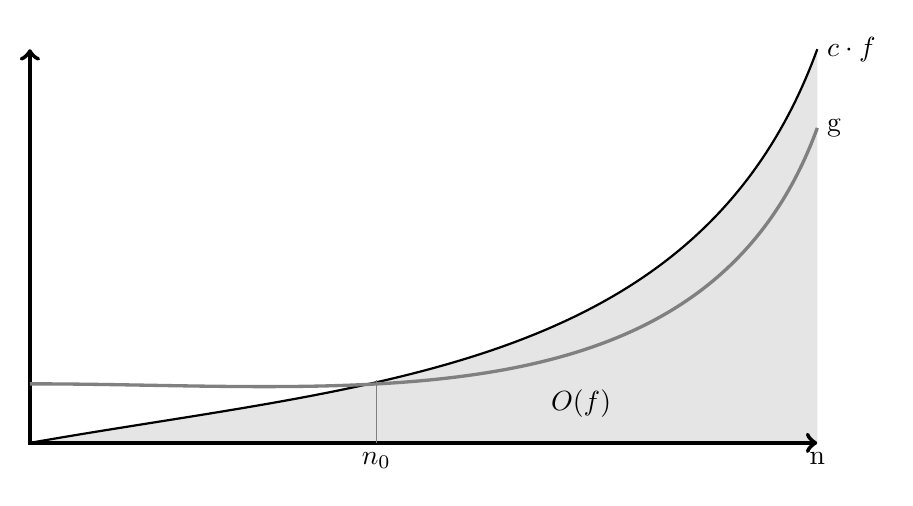
\begin{tikzpicture}

%\draw (0,0) grid (10,5);

\path [fill=white!90!black]  (0,0) to [out=10, in=250] (10,5) -- (10,0) -- (0,0);
\draw [<->, ultra thick] (0,5) -- (0,0) -- (10,0);
\node [below] at (10,0) {n};
\draw [thick] (0,0) to [out=10, in=250] (10,5); \node [right] at (10,5) {$c\cdot f$};

\draw [very thick,gray] (0,0.75) to [out=0, in=250] (10,4); \node [right] at (10,4) {g};

\node [below] at (4.4,0) {$n_0$}; \draw [help lines] (4.4,0) -- (4.4,0.8);
\node at (7,0.5) {$O(f)$};

\end{tikzpicture}

$g(n)\leq c \cdot f(n)$ für große $n$.
$g \in O(f)$

Beispiel: $17n^2 + 3n + 5\log(n) \in O(n^2)$, da
$17n^2 + 3n + 5\log(n) \leq 17n^2 + 3n^2 + 5n^2= \underbrace{25}_{c} n^2$ für alle $n >0$

Ziel ist es, stets eine möglichst gute und einfache Abschätzung anzugeben. 

Typische Laufzeiten:
\begin{itemize}

\item $O(1):$ Konstante Laufzeit\\
Beispiel:
\begin{lstlisting}[numbers=left, tabsize=4, style=customc]
a=1;
b=2;
c=3;
\end{lstlisting}
LF insgesamt: $3 \cdot c \leq 1 \cdot (3 \cdot c) \in O(1)$

\item $O(n):$ Lineare Laufzeit

\item $O(2^n):$ Brute-Force-Algorithmen

\end{itemize}

\paragraph{Graphen}
Königsberger Brückenproblem
%Todo Zeichnung Foto 2013-11-13T09:26
Gibt es einen Rundweg der über jede Brücke genau einmal führt?

Graph zum Königsberger Brückenproblem

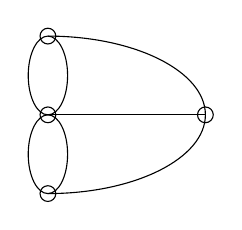
\begin{tikzpicture}
\draw (0,2) circle [radius=0.1];
\draw (0,1.5) circle [y radius=0.5,x radius=0.25]; \draw (2,1) arc [x radius=2, y radius =1, start angle = 0, end angle= 90];
\draw (0,1) circle [radius=0.1]; \draw (0,1) -- (2,1);   \draw (2,1) circle [radius=0.1];
\draw (0,0.5) circle [y radius=0.5,x radius=0.25]; \draw (0,0) arc [x radius=2, y radius =1, start angle = -90, end angle= 0];
\draw (0,0) circle [radius=0.1];

\end{tikzpicture}
%Todo Zeichnung Foto 2013-11-13T09:28

\subparagraph{Definition} Ein (ungerichteter) Graph ist ein Paar $G=(V,E)$, wobei
\begin{itemize}
\item $V$ die Menge der Knoten ist
\item $E$ die Menge der Kanten ist, die aus ungeordneten Paaren $\{U,V\}$ von Knoten besteht.
\end{itemize}

Beispiel:
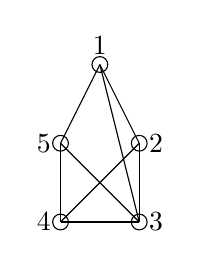
\begin{tikzpicture}
\draw (0.5,2) circle [radius=0.1]; \node [above] at (0.5,2) {1};
\draw (1,1) circle [radius=0.1]; \node [right] at (1,1) {2};
\draw (1,0) circle [radius=0.1]; \node [right] at (1,0) {3};
\draw (0,0) circle [radius=0.1]; \node [left] at (0,0) {4};
\draw (0,1) circle [radius=0.1]; \node [left] at (0,1) {5};
\draw (0.5,2) -- (1,1); \draw (1,1) -- (1,0); \draw (1,0) -- (0,0); \draw (0,0) -- (0,1); \draw (0,1) -- (0.5,2);
\draw (1,1) -- (0,0);
\draw (1,0) -- (0,1);
\draw (0.5,2) -- (1,0);


\end{tikzpicture}

$G=(\{1,2,3,4,5\},\{\{1,2\},\{1,3\},\{1,5\},\{2,3\},\{2,4\},\{3,4\},\{4,5\},\{3,5\}\})$

\subparagraph{Definition} Ein Graph heißt vollständig, wenn alle Knoten paarweise verbunden sind.\\
Folgerung: Ein vollständiger Graph mit $n$ Knoten besitzt $\binom{n}{2}$ Kanten.

\subparagraph{Definition} Ein Knoten $v$ hat den Grad $k$, wenn $v$ mit genau $k$ anderen Knoten verbunden ist.\\
Notation: $deg(v)=k$
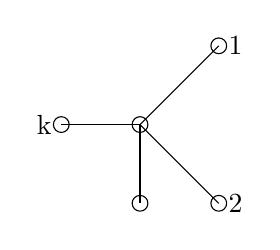
\begin{tikzpicture}
\draw (0,0) circle [radius=0.1];
\draw (1,1) circle [radius=0.1];
\draw (-1,0) circle [radius=0.1];
\draw (1,-1) circle [radius=0.1];
\draw (0,-1) circle [radius=0.1];
\node [right] at (1,1) {1};
\node [right] at (1,-1) {2};
\node [left] at (-1,0) {k};
\draw (0,0) -- (1,1);
\draw (0,0) -- (-1,0);
\draw (0,0) -- (1,-1);
\draw (0,0) -- (0,-1);

\end{tikzpicture}



\subparagraph{Satz} (Handshake Lemma)\\*
Für jeden Graphen $(V,E)$ gilt $\sum\limits_{v\in V} deg(v)=2\lvert E\rvert$

Beweis: Wenn wir jede Kante in der Mtite durchschneiden, ist jeder Knoten $v$ mit genau $deg(v)$ Hälften verbunden. Also ist $\sum\limits_{v\in V} dev(v)$ gleich der Anzahl der Kantenhälften und diese ist $2\lvert E \rvert$.

\paragraph{Weg und Kreise}
\subparagraph{Definition}
Ein Weg (von $v_1$ nach $v_k$) ist eine endliche Folge von Knoten $v_1,...,v_k$ mit $\{v_l,v_{l+1}\} \in E$ für $l=1,...,k=1$

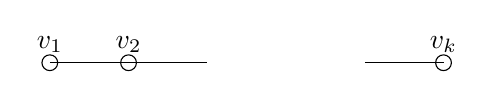
\begin{tikzpicture}
\draw (0,0) circle [radius=0.1]; \node [above] at (0,0) {$v_1$};
\draw (0,0)--(1,0);
\draw (1,0) circle [radius=0.1]; \node [above] at (1,0) {$v_2$};
\draw (1,0)--(2,0);
\draw (5,0) circle [radius=0.1]; \node [above] at (5,0) {$v_k$};
\draw (4,0)--(5,0);
\end{tikzpicture}

Ein Weg heißt Kreis, wenn $v_1 = v_r$.\\
Ein Graph heißt zusammenhängend, wenn es für alle Paare von Knoten $u,v$ einen Weg von $u$ nach $v$ gibt.\\
Ein Pfad ist ein Weg, der keine Knoten mehrfach enthält.

Beispiel\\
Ein Hamiltonkreis ist ein Kreis, der jeden Koten genau einmal enthält.\\
%Todo Zeichnung 2013-11-13T10:20
Für einen Graphen $G$ ist ein Euler-Kreis ein Kreis, der jede Kante genau einmal enthält.
\subparagraph{Satz} (Euler)\\*
Ein zusammenhängender Graph besitzt einen Euler-Kreis genau dann, wenn der Grad aller Knoten gerade ist.
(Königsberger Brückenproblem nicht lösbar)

\paragraph{Bäume}
Definition: Ein Baum ist ein zusammenhängender Graph, der keine Kreise enthält. Ein Blatt ist ein Knoten $v$ mit $deg(v)\leq 1$.

Satz: Sei $G=(V,E)$ ein Baum. Dann besitzt $G \; \lvert V \rvert -1$ Kanten.\\
Beweis (Induktion nach $n=\lvert V \rvert$ )\\*
$n=1:$ Ein Baum mit einem Knoten besitzt 0 Kanten.\\
$n \rightarrow n+1:$ Sei $G$ ein Baum mit $n+1$ Knoten. $G$ besitzt ein Blatt (s. HA). Wenn wir in $G$ ein Blatt zusammen mit der zugehörigen Kante entfernen, erhalten wir einen Baum $G'$ mit $n$ Knoten und nach Induktionsvorraussetzung $n-1$ Kanten. Wenn wir die abgerissene Kante wieder hinzufügen, erhalten wir den Baum $G$ und dieser besitzt $n-1 +1 = n$ Kanten.

\subparagraph{Definition} Ein binärer Wurzelbaum ist ein Baum, in dem jeder Knoten, der kein Blatt ist, genau zwei Nachfolger besitzt.\\
Ferner ist genau ein Knoten als Wurzel ausgezeichnet.

 
Satz: Sei $B$ ein binärer Wurzelbaum, in dem jeder Pfad von der Wurzel zu einem Blatt die Länge $k$ hat. Dann besitzt $B$ genau $2^k$ Blätter.

Beweis (Induktion nach $k$)\\*
$k=0:$ Ein Binärbaum, der nur aus der Wurzel besteht, besitzt $2^0=1$ Blatt.\\*
$k \rightarrow k+1:$ Wir betrachten einen Binärbaum der Tiefe $k=1$. Jeder der beiden Teilbäume, die sich unter der Wurzel befinden, sind selbst binäre Wurzelbäume.
%Todo 2013-11-27T10:13
Da diese jeweils die Tiefe $k$ besitzen, folgt aus der Induktionsvorraussetzung, dass diese Teilbäume jeweils $2^k$ Blätter besitzen. Folglich besitzt der Binärbaum der Tiefe $k=1, \; 2 \cdot 2^k = 2^{k+1}$ Blätter.

\paragraph{Algorithmus}
Ein Algorithmus ist ein Verfahren, um ein Problem in einer endlichen Anzahl von Schritten zu lösen. Ein Algorithmus kann in einer Programmiersprache implementiert werden.

Suchverfahren: Bereits behandelt: Lineare Suche, Laufzeit $O(n)$

Binäre Suche: Vorraussetzung: Sortiertes Array.\\
Bei der binären Suche wird nach einem Wert $x$ gesucht, indem zunächst $x$ mit dem Wert in der Mitte des Arrays verglichen wird. Wenn der Wert gefunden wurde, ist der Algorithmus fertig. Sonst wird auf gleiche Weise weitergesucht in der 
\begin{itemize}
\item linken Hälfte des Array, wenn der gesuchte Wert kleiner als der Wert in der Mitte des Arrays
\item rechten Hälfte des Array, wenn der gesuchte Wert größer als der Wert in der Mitte des Arrays
\end{itemize}
ist.\\
Beispiel: Suche nach $17$ in dem Array\\
$
\begin{array}{|c|c|c|c|c|c|c|c|c|c|}
\hline
0 & 1 & 2 & 3 & 4 & 5 & 6 & 7 & 8 & 9\\ \hline
2 & 5 & 6 & 7 & 10 & 16 & 22 & 30 & 31 & 50\\
\hline
\end{array}$

Analyse der Laufzeit: Wir stellen das Verhalten der binären Suche bei erfolgloser Suche als Binärbaum dar.\\
Ferner nehmen wir $n=2^k$ an. Dabei entsprechen den Knoten die von der binären Suche ausgeführte Vergleiche, die Kanten dem Weitersuchen im linken bzw. rechten Teilarray.\\
Da in jedem Durchlauf des Algorithmus ein konstanter Aufwand für den Vergleich und das Bestimmen der Teilarrays entsteht, ist die Laufzeit $O(\text{Anzahl Durchläufe})$. Die Anzahl der Durchläufe ist die Länge des längsten Pfades von der Wurzel zu einem Blatt.
Da jedes Blatt einem Teilarray mit einem Element entspricht, gibt es genau $n$ Blätter.

Aus dem oben bewiesenen Satz folgt, dass dieser Binärbaum daher die Tiefe $k = \log_{(2)}{n}$ besitzt.\\
Die Laufzeit der binären Suche liegt folglich in $O(\log{n})$.

\subparagraph{Binäre Suchbäume}
Um auch in dynamischen Datenstrukturen zu suchen, lassen sich Suchbäume verwenden. Ein Suchbaum ist ein Binärbaum für den gilt:\\
Jeder in ein Knoten gespeicherter Wert ist größer als alle Werte im linken Teilbaum und kleiner als alle Werte im rechtem Teilbaum.\\*
\Tree [.5 [.3 2 4 ] [.8 6 9 ] ]
\\
Implementierung in C
%Todo 2013-12-11T09:36

Zur Verwendung eines binären Suchbaumes (jeder Knoten hat $\leq 2$ Blätter) sind folgende Funktionen nötig:
\begin{itemize}
\item Suche nach einen Wert\\
Dazu wird der Suchbaum, beginnend an der Wurzel, rekursiv durchsucht.
Die Laufzeit ist von der Tiefe des Baums abhängig. Bei einem vollständig balancierten Baum liegt diese in $O(\log{n})$, bei einem linear entarteten Baum in $O(n)$.
\item Werthinzufügen\\
Dazu wird der Baum wie oben durchsucht. Wenn der Wert bereits vorhanden ist, wird die Funktion beendet. Ansonsten wird ein Blatt mit dem neuen Wert hinzugefügt unter dem zulest von der Suche besuchten Knoten (links oder rechts).
LZ: Wie Suche.
\item Wert entfernen: Kompliziert
\end{itemize}

\subparagraph{Hashing} Gegeben: Eine Menge $U$ von potenziellen Schlüsseln (z.B. Artikelnummer), Menge $S\subseteq U$ von zu verwaltenden Schlüsseln.\\
Zur Verwaltung der Datensätze wird eine Hashfunktion $h: U \mapsto T$ verwendet, die in eine Hashtabelle $T$ abbildet.
Wenn wir annehmen, dass h injektiv wäre,\\*
dann lassen sich folgende Operationen implementieren:
\begin{itemize}
\item Suche if(T[h(s)] $>$ 0)
\item Einfügen T[h(s)]++
\item Löschen T[h(s)]=0
\end{itemize}
Wegen $\lvert U \rvert >> \lvert S \rvert$ kann $h$ aber nicht injektiv sein (Schubfachprinzip). Folglich sind Kollisionen möglich, d.h. zwei unterschiedliche Schlüssel $s,s'$ können den gleichen Hashwert $(h(s)=h(s'))$ besitzen.

Einfache Lösung zur Behandlung von Kollisionen: Überlauflisten\\*
Eine Liste ist eine dynamische Datenstruktur, bei der jedes Element der Liste einen Verweis auf ein nachfolgendes Listenelement enthält.

\begin{tikzpicture}
\draw [->,thick] (0,0) -- (1,0); \draw (1,-0.5) rectangle   (1,1);
\draw [->,thick] (3,0) -- (4,0); \draw (4,-0.5) rectangle   (1,1);
\draw [->,thick] (6,0) -- (7,0); \draw (7,-0.5) rectangle   (1,1);
\draw [->,thick] (9,0) -- (10,0); \draw (10,-0.5) rectangle (1,1);


\end{tikzpicture} %Todo 2013-12-11T10:49

Implementierung in C durch structs und Zeiger\\
Laufzeit Zugriff auf ein Listenelement $O(n)$.

Um Überlauflisten zu verwenden, verwenden wir eine Tabelle von Listen. An jeder Position der Hashtabelle werden die dort gespeicherten Einträge in einer Liste verwaltet.\\
Wenn die Hashtabelle nicht zu stark befüllt ist (z.B. Anzahl gespeicherte Elemente $n=\frac{1}{2}$), dann sind alle Hashoperationen im Mittel in der Zeit $O(1)$ möglich.\\
Mögliche Hashfunktion $h(s)=s \mod{m}$

Weitere Anwendungen von Hashing: Digitale Unterschrift.\\
Prinzip: Ein Dokument oder ein Programmtext wird als (sehr große) Zahl betrachtet, z.B. in dem die Zeichen (Bytes) hintereinander geschrieben als Zahl zu einer geeigneten Basis betrachtet wird. Auf diese Zahl wird eine Hashfunktion angewendet. Der Hashwert ist die Signatur des Dokumentes.

\begin{tikzpicture}
\draw (0,0) rectangle (4,4); \draw [->,thick] (4,2) -- (6,2); \draw (6,1) rectangle (8,3); \node at (2,3) {Programm P}; \node [above] at (5,2) {$h(p)$}; \node at (7,2) {Signatur S};
\end{tikzpicture}\\
Damit lässt sich Prüfen ob das Programm $P$ zu der Signatur $S$ passt.

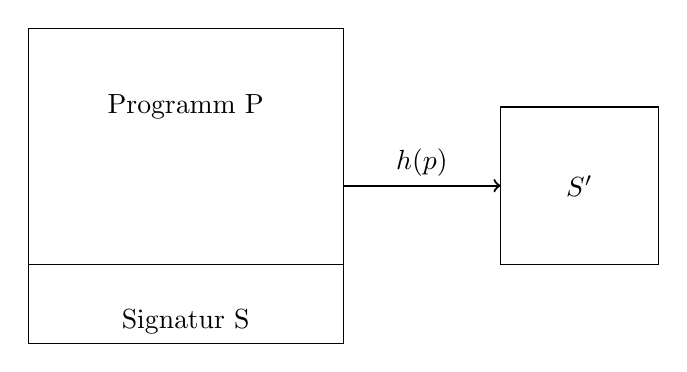
\begin{tikzpicture}
\draw (0,1) rectangle (4,4); \draw [->,thick] (4,2) -- (6,2); \draw (6,1) rectangle (8,3); \node at (2,3) {Programm P}; \node [above] at (5,2) {$h(p)$}; \node at (7,2) {$S'$};
\draw (0,0) rectangle (4,1); \node [above] at (2,0) {Signatur S};
\end{tikzpicture}\\
Für $S = S'$ wurde $P$ nicht verändert. Für $S \neq S'$ ist $P$ fehlerhaft (möglich Ursachen: Fehler bei der Datenübermittlung, $P$ wurde manipuliert).\\
Anwendung: Integritätsprüfung von Programmen in der Linux-Paketverwaltung.\\
Schutz vor Veränderung von Hardware oder Systemeinstellungen. (Digital Rights Managment, Motorsteuergeräte)\\
Notwendig ist dazu eine (möglichst) kollisionsresistente Hashfunktion. Denn wenn ein Angreifer einen Schadcode $P'$ erzeugen kann, mit $h(P)=h(P')$, dann kann dies durch das Prüfen des Hashwertes nicht festgestellt werden.

\subparagraph{Sortierverfahren}
Naive Sortierverfahren haben eine Laufzeit in $O(n^2)$. Ein besseres Verfahren ist Quicksort führt rekursiv zwei Schritte aus:
\begin{enumerate}
\item Ein beliebiges Element des zu sortierenden Feldes wird als Pivotelement ausgewählt. Bei Listen wird das erste Element verwendet, weil der Zugriff darauf in Zeit $O(1)$ möglich ist.\\
\begin{tikzpicture}
\draw (0,0) rectangle (2,2); \draw (2,0) rectangle (10,2);
\node [below] at (1,0) {Pivotelement}; \node [below] at (5,0) {Rest der Liste};
\end{tikzpicture}
\item Die Elemente werden so umgeordnet das die Elemente $\leq$ Pivotelement vorne, die Elemente $>$ Pivotelement hinten und dazwischen das Pivotelement stehen.
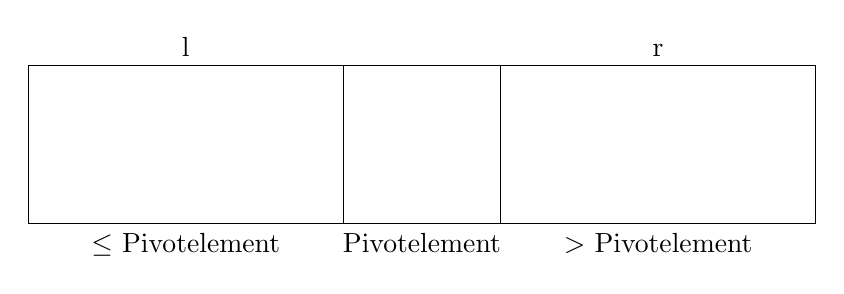
\begin{tikzpicture}
\draw (0,0) rectangle (4,2); \draw (4,0) rectangle (6,2); \draw (6,0) rectangle (10,2);
\node [above] at (2,2) {l}; \node [above] at (8,2) {r};
\node [below] at (2,0) {$\leq$ Pivotelement}; \node [below] at (8,0) {$>$ Pivotelement}; \node [below] at (5,0) {Pivotelement};
\end{tikzpicture}
\item Quicksort wird rekursiv für die Listen l,r aufgerufen, bis die Liste leer ist.
\end{enumerate}
Die Laufzeitanalyse von Quicksort ist schwierig, da die Teillisten l,r unterschiedliche Längen haben können. Wir betrachten dazu ein ähnliches Sortierverfahren: Mergesort.\\
Mergesort sortiert wie folgt:
\begin{enumerate}
\item Die zu sortierende Liste (bzw. das Array) wird halbiert. Es entstehen Teillisten l,r.
\item Die Teillisten l,r werden rekursiv sortiert, bis sie leer oder die Länge 1 haben.
\item Die sortierten Teillisten werden zu einer sortierten Liste zusammengefügt (Merge-Operation).
\end{enumerate}

Laufzeitanalyse von Mergesort\\
Wir stellen das Verhalten von Mergesort für $n=2^k$ als Binärbaum dar:\\
\Tree [. [.$\frac{n}{2}$ [.$\frac{n}{4}$ $\vdots$ $\vdots$ ] [.$\frac{n}{4}$ $\vdots$ $\vdots$ ] ][.$\frac{n}{2}$ [.$\frac{n}{4}$ $\vdots$ $\vdots$ ] [.$\frac{n}{4}$ $\vdots$ $\vdots$ ] ] ]\\
Zum Erzeugen der Hälften und den Zusammenfügen fällt der Aufwand $O(\lvert\text{linke Hälfte}\rvert + \lvert\text{rechte Hälfte}\rvert )$ an.\\
Auf jeder Ebene des Baumes sind das $O(n)$. Die Tiefe des Baumes ist $n$. Satz aus der Vorlesung $k=\log{n}_2$. Die Laufzeit von Mergesort liegt folglich in $O(n \log{n})$.\\
Dies liegt nahe am theoretischen Optimum für Sortierverfahren.

Die mittlere Laufzeit von Quicksort liegt ebenfalls in $O(n \log{n})$.\\
Worstcase Laufzeit von Quicksort:\\
Wir stellen die rekursiven Aufrufe von Quicksort für eine sortierte Liste als Binbaum dar:\\
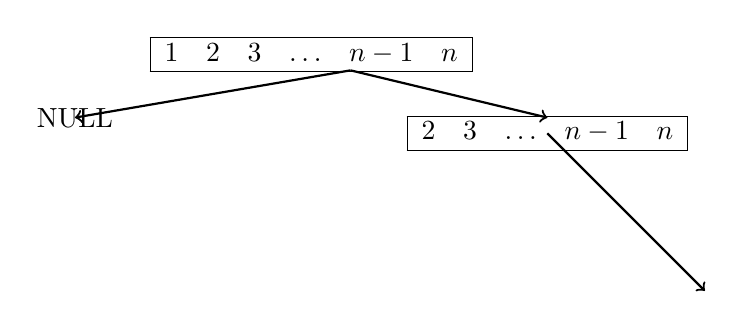
\begin{tikzpicture}
\node at (0,0) {$\begin{array}{|cccccc|}\hline 1 & 2 & 3 & \dots & n-1 & n\\ \hline \end{array}$}; \draw [->,thick] (0.5,-0.2) -- (3,-0.8); \draw [->,thick] (0.5,-0.2) -- (-3,-0.8);
\node at (-3,-0.8) {NULL};
\node at (3,-1) {$\begin{array}{|ccccc|}\hline 2 & 3 & \dots & n-1 & n\\ \hline \end{array}$}; \draw [->,thick] (3,-1) -- (5,-3);
\end{tikzpicture}\\
Anzahl der Vergleiche beim Sortieren einer sortierten Liste:\\
$n-1 + n-2 + ... + 1 = \frac{(n-1)n}{2} \in O(n^2)$\\
Die Laufzeit von Quicksort für eine sortierte Liste liegt daher in $O(n^2)$.\\
\begin{tikzpicture}[yscale=0.2, xscale=2]
\draw [->,very thick] (1,0) -- (1,25); \node [left] at (1,25) {y};
\draw [->,very thick] (1,0) -- (5,0); \node [below] at (5,0) {x};

\node [below] at (1,0) {1}; 

\draw [domain=1:5] plot (\x, {pow(\x,2)});
\draw [domain=1:5] plot (\x, {\x * log2(\x)});%Todo
\end{tikzpicture}

Platzbedarf:\\
Quicksort kann ohne zusätzlichen Speicherplatz (in-place) implementiert werden.\\
Mergesort braucht zusätzlichen Speicherplatz für die Merge-Operation.

\subparagraph{Graphalgorithmen}
Datenstrukturen zur Repräsentation von Graphen:
\begin{itemize}
\item Adjazenzmatrix: Die ist eine Matrix $(a_{uv})$ mit $a_{uv} = \left\{ \begin{array}{rcl}
         1
         & \mbox{für}
         & \{u,v\} \in E \\ 
        0
         & \mbox{sonst} \\
                \end{array}\right.$ 
                
\item Adjasenzliste: Array, das an der Position $u\in V$ eine Liste aller Knoten  $v\in V$ enthält mit $\{u,v\} \in E$
\end{itemize}
%Todo siehe 2014-01-08T10:10
Speicherbedarf:\\
Adjazenzmatrix $O(\lvert V \rvert^2)$\\*
Adjazenzliste $O(\lvert V \rvert + \lvert E \rvert)$\\
Für Bäume verbraucht die Adjazenzliste den Platz $O(\lvert V \rvert + \lvert V \rvert -1) = O(\lvert V \rvert )$ und damit weniger Platz als die Adjazenzmatrix.\\
Für beliebige Graphen gilt ferner $O(\lvert V \rvert + \lvert E \rvert ) \subseteq O(\lvert V \rvert \frac{\lvert V \rvert \cdot \lvert V-1 \rvert }{2}) = O(\lvert V \rvert^2 )$.

\begin{tabular}{l|c|c}
Rechenzeit: & Adjazenzmatrix & Adjazenzliste\\ \hline
Feststellen ob $\{ u,v \} \in E$ & $O(1)$ & $O(\deg{u})$\\
Nachbarn eines Knotens $u$ bestimmen & $O(\lvert V \vert)$ & $O(\deg{u} )$\\
\end{tabular}\\
Folgerung: Adjazenzliste meistens effizienter als Adjazenzmatrix.

\subparagraph{Breitensuche}
Die Breitensuche durchsucht alle Knoten eines Graphen, beginnend mit einem Startknoten, indem schichtweise die Nachbarn eines Knotens, danach die Nachbarn dieser Knoten usw. besucht werden.

Beispiel: Breitensuche in einem Wurzelbaum\\
Die Suche beginnt im Knoten $s$ (Zahl gibt Reihenfolge des Besuchs an)\\
\Tree [.s(1) [.2 5 6 ] [.3 [.7 10 11 12 ] 8 ] [.4 [.9 13 14 ] ] ]

\subparagraph{Tiefensuche} Die Tiefensuche durchsucht alle Knoten eines Graphen, beginnend mit einem Startknoten, indem Pfade verfolgt werden, bis ein Knoten keine unbesuchten Nachbarn mehr besitzt. Erst wenn das Ende eines Pfades erreicht ist, werden unbesuchte Nachbarn des zuletzt besuchten Knotens besucht (Backtracking).

Beispiel: Tiefensuche in einem Wurzelbaum\\
\Tree [.s(1) [.2 3 4 ] [.5 [.6 7 8 9 ] 10 ] [.11 [.12 13 14 ] ] ]

Warteschlange: \textsc{FIFO}-Datenstruktur (First in, first out)\\
Entnehmen $\leftarrow \begin{array}{|c|c|c|c|c|c|c|}
\hline &&&&&& \\ \hline \end{array} \leftarrow $ Einfügen\\
Effiziente Implementierung: Einfach verkette Liste mit zusätzlichen Zeiger auf das letzte Element\\
$\rightarrow \begin{array}{|c|} \hline \\ \hline \end{array} \rightarrow \begin{array}{|c|} \hline \\ \hline \end{array} \rightarrow \begin{array}{|c|} \hline \\ \hline \end{array} \rightarrow \begin{array}{|c|} \hline \\ \hline \end{array} \leftarrow$\\
Entnehmen $O(1)$

Algorithmus Breitensuche (für zusammenhängende Graphen)
\begin{enumerate}
\item Füge Startknoten einer Warteschlange hinzu
\item Solange die Warteschlange nicht leer ist:
\begin{itemize}
\item Entferne das erste Element $v$ von der Warteschlange
\item Füge noch unbesuchte Nachbarn von $v$ der Warteschlange hinzu
\end{itemize}
\end{enumerate}
Beispiel:\\
\Tree [.1 [.2 4 5 ] 3 ] \\*
$\begin{array}{|c|} \hline 1\\ \hline \end{array}$\\*
$\begin{array}{|c|c|} \hline 2 & 3\\ \hline \end{array}$\\*
$\begin{array}{|c|c|c|} \hline 3 & 4 &  5\\ \hline \end{array}$\\*
$\begin{array}{|c|c|} \hline 4 & 5\\ \hline \end{array}$\\*
$\begin{array}{|c|} \hline 5\\ \hline \end{array}$\\*
\textsc{NULL}

Laufzeit: Jeder Knoten $v$ wird genau einmal aus der Warteschlange entfernt und für $\deg{v}$ Nachbarn geprüft, ob diese in die Warteschlange eingefügt werden müssen. Aufwand dazu, wenn eine Adjazenzliste verwendet wird:
\[ O(\sum\limits_{v \in V} (1+ \deg{v})) = O(\lvert V \rvert + \sum\limits_{v \in V} \deg{v} ) = O(\lvert V \rvert + 2 \lvert E \rvert ) \overbrace{=}^{\text{Handshake-L.}} O(\lvert V \rvert +  \lvert E \rvert ) \]

Tiefensuche: Aus der Implementierung der Breitensuche erhalten wir eine Tiefensuche, wenn anstelle der Warteschlange ein Stack verwendet wird.\\
Stack: \textsc{LIFO}-Datenstruktur (Last in, first out)\\
$
\; \updownarrow \\*
\begin{array}{|c|} 
\\ \hline
\\ \hline
\\ \hline
\\ \hline
\\ \hline
\end{array}$\\
Ein Stack kann durch eine einfach verkettete Liste realisiert werden.\\*
Einfügen, Entnehmen: $O(1)$

Beispiel:\\
\Tree [.1 [.2 4 5 ] 3 ] \\*
--\\*
$\begin{array}{|c|} 
1 \\ \hline
\end{array}$\\*
--\\*
$\begin{array}{|c|} 
2\\ \hline
3\\ \hline
\end{array}$\\*
--\\*
$\begin{array}{|c|} 
4\\ \hline
5\\ \hline
3\\ \hline
\end{array}$\\*
--\\*
$\begin{array}{|c|} 
5\\ \hline
3\\ \hline
\end{array}$\\
Laufzeit: Gleiche Laufzeit wie die Breitensuche, da nur die Reihenfolge, in der die Knoten besucht werden, unterschiedlich ist.\\

\paragraph{Gerichtete Graphen und binäre Relationen}
\subparagraph{Definition} Ein gerichteter Graph ist ein Paar $G=(V,E) \text{ mit } E \subseteq V \times V$.

Beispiel: $G=(V,E) \text{ mit } V = \{ 1,2,3\}, E=\{ (1,1),(1,2),(2,1),(2,3)\}$\\
$1_\circlearrowleft \leftrightarrow 2 \rightarrow 3$

\subparagraph{Definition} Sei $E$ eine binäre Relation auf $V$ (d.h. $E \subseteq V \times V$).
\begin{itemize} %Todo 2014-01-15T10:22
\item Die reflexive Hülle von $E$ ist die Relation $E \cup \{ (v,v) | v \in V\}$
\item Die symmetrische Hülle von $E$ ist die Relation $E \cup \{(v,u) | (u,v) \in E\}$
\item Die transitive Hülle von $E$ ist die Relation \[\bigcup\limits_{n\geq 1} E^n\] oder gleichwertig \[ E\cup \{ (v,w) | \exists v_1, \dots v_k \in V: (v,v_1) \in E, (v_1,v_2) \in E, \dots , (v_k,w) \in E \}\]
\item Die reflexive und transitive Hülle von $E$ ist die Vereinigung der reflexiven und der transitiven Hülle von $E$.%Todo 2014-01-15T10:35
\item Aus den Labyrinth kann ein Graph $G=(V,E)$ erzeugt werden. Daraus kann man einen gerichteten Graphen $G' = (V,E')$ mit $E' = \{(u,v) | \{u,v\} \in E \} \cup \{ (v,u) | \{u,v\} \in E \}$ erzeugen.\\
Es gibt einen Weg zum Ausgang, wenn (Startposition, Ausgangsknoten) $\in$ reflexiv-transitive Hülle von $E'$.\\
Die reflexiv-transitive Hülle einer Relation lässt sich mit einer Breiten- oder Tiefensuche berechnen.
\end{itemize}

\paragraph{Topologische Sortierung}
\subparagraph{Problem} Wie lassen sich Arbeitsschritte, zwischen denen eine Abhängigkeit besteht, in eine Reihenfolge bringen?

\subparagraph{Definition} Sei $G=(V,E)$ ein DAG (directed acyclic graph).\\
Eine topologische Sortierung von $G$ ist eine Nummerierung von $G$ mit Nummer $(n) < $ Nummer $(r)$ für $(u,v) \in E$.

Beispiel: Eine topologische Sortierung kann durch eine Tiefensuche bestimmt werden:

\begin{lstlisting}[mathescape,numbers=left, tabsize=4, style=customc]
topsort:
    for v $\in$ V
        markiere v mit weiss
    for v $\in$ V
        tiefensuche(v)
        
tiefensuche(v):
    v grau: Fehler ("Graph enthaelt Kreis")
    v weiss: markiere v mit grau
        for $\{ u | (v,u) \in E \}$
            tiefensuche(u)
        markiere v mit schwarz und fuege v an den Kopf einer Liste
\end{lstlisting}

Laufzeit: $O(\lvert V \rvert + \lvert E \rvert)$ (wie bei Tiefensuche)

\paragraph{Codierungstheorie} 
\subparagraph{Problem} Daten können bei der Übertragung verändert werden. Wie können die Fehler erkannt und gegebenenfalls korrigiert werden?\\
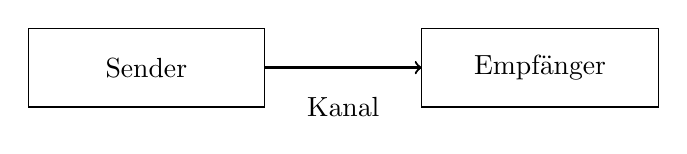
\begin{tikzpicture}
\draw (0,0) rectangle (3,1); \node at (1.5,0.5) {Sender}; 
\draw [->,thick] (3,0.5) -- (5,0.5); \node at (4,0) {Kanal}; %Todo Über Kanal \Blitz Störung
\draw (5,0) rectangle (8,1); \node at (6.5,0.5) {Empfänger};
\end{tikzpicture}\\
Häufige Lösung zur Fehlererkennung: Prüfsummen

\subparagraph{Paritätsprüfung} Für eine Folge von Bits $b_1,\dots, b_{n-1} \in \{ 0,1\}$ wird das Paritätsbit 
\[ b_n = ( \sum\limits_{i=1}^{n-1} b_i) \mod{2} \]
berechnet. Das erhaltene Codewort ist $b_1,\dots,b_n$.

Beispiel:\\
$00000$ ist ein Codewort\\
$00001$ ist kein Codewort\\
$10100$ ist ein Codewort\\
$11100$ ist kein Codewort\\

In der endlichen Gruppe $\mathbb{Z}_2,t) \text{ gilt } 1+1 \equiv 0 ( \mod{2})$. Aus
\[ \sum\limits_{i=1}^{n-1} b_i \equiv b_n (\mod{2})\]
folgt daher
\[ \sum\limits_{i=1}^{n} b_i \equiv 0 (\mod{2} )\]
Die Menge der Codewörter lässt sich damit darstellen durch
\[\{ (b_1,\dots,b_n)\in \{ 0,1\}^n | \sum\limits_{i=1}^{n} b_i \equiv 0 (\mod{2} ) \} \]

Satz: Der Parity-Check-Code ist 1-fehlererkennend.

Beweis: Seien $b_1,\dots,b_n$ ein Codewort und $b'_1,\dots,b'_n$ ein Wort, das sich an Stelle $k$ von $b_1,\dots,b_n$ unterscheidet. Angenommen $b'_1,\dots,b'_n$ ist ein Codwort. Dann gilt $0 \equiv \sum\limits_{i=1}^{n} b'_i \equiv \sum\limits_{i=1}^{n} b_i + (b'_k - b_k) \equiv 0 + b'_k - b_k \equiv \underbrace{1}_{\text{da } b'_k \neq b_k}$ Widerspruch, q.e.d.

Anwendungen
\begin{itemize}
\item Fehlererkennung in Hardware (Speicher, Festplatte, Netzwerke)
\item 7-bit ASCII (Bit 8 als Paritätsbit)
\end{itemize}
Ferner kann das Verfahren zur Rekonstrutktion eines verloren gegangenen Bits verwendet werden, wenn die restlichen Bits fehlerfrei sind.\\
Denn aus
\[ 0 \equiv \sum\limits_{i=1}^{n} b_i (\mod{2})\]
folgt für $1 \leq k \leq n$
\[b_k \equiv \sum\limits_{i \neq k} b_i (\mod{2})\]
Damit kann Bit $b_k$ aus den anderen Bits rekonstruiert werden.

Anwendung: \textsc{Raid4} \textsc{Raid5}

Daten und Parität werden auf $n$ Festplatten verteilt. Beim Ausfall einer Platte können die Daten rechnerisch rekonstruiert werden.

\subparagraph{\textsc{ISBN}-Code} Um festzustellen, ob eine Buchnummer falsch eingetippt wurde, enhält der \textsc{ISBN}-Code eine Prüfsumme.\\
Beispiel: $\underbrace{382741826}_{9\text{-st. BuchNr}}\underbrace{7}_{\text{Prüfziffer}}$\\
Für die Prüfziffer gilt:\\
$z_{10} = \sum\limits_{i=1}^{9} (i \cdot z_i ) \mod{11}$\\
Dabei wird $X$ für den Wert $10$ verwendet.

Wegen $10+1 \equiv 0 (\mod{11})$ ist $10$ das inverse Element zu $1$ bezüglich $+$ (d.h. $10$ entspricht $-1$). Aus obiger Gleichung folgt damit
\[ 0 \equiv \sum\limits_{i=1}^{10} i \cdot z_i (\mod{11})\]
Die Menge der Codewörter ist daher
\[\{ (z_1,\dots,z_{10}) | z_1,\dots,z_9 \in \{ 0,\dots,9\},z_{10} \in \{0,\dots,10\}, \sum\limits_{i=1}^{10} i \cdot z_1 \equiv 0 (\mod{11}) \}\]

\subparagraph{Satz} Der \textsc{ISBN}-Code ist 1-fehlererkennend.

Beweis: Seien $z_1,\dots,z_{10}$ ein Codewort und $z'_1 \dots z'_{10}$ ein Wort, das sich an Stelle $k$ von $z_1,\dots,z_{10}$ unterscheidet. Angenommen $z'_1 \dots z'_{10}$ ist ein Codewort. Dann gilt
\[0 \equiv \sum\limits_{i=1}^{10} i \cdot z'_i \equiv \sum\limits_{i=1}^{10} i \cdot z_1 + k \cdot (z'_k - z_k) \equiv 0 + k (z'_k - z_k)\]
Da $11$ eine Primzahl ist, ist $(\mathbb{Z}_{11},+,\cdot)$ ein Körper. Daher können wir durch $k$ teilen und erhalten
\[ 0 \equiv z'_k - z_k \]
woraus $z'_k \equiv z_k$ folgt, Widerspruch, q.e.d.

\subparagraph{Satz} Der \textsc{ISBN}-Code erkennt Vertauschungen von Ziffern (insbesondere Zahlendreher) ohne Beweis.

\paragraph{Fehlerkorrigierende Codes} Idee: Für ein empfangenes Wort $w$ suchen wir ein Codewort $v$, so dass der Abstand $d(v,w)$ minimal ist. (nearest neighbor decoding).

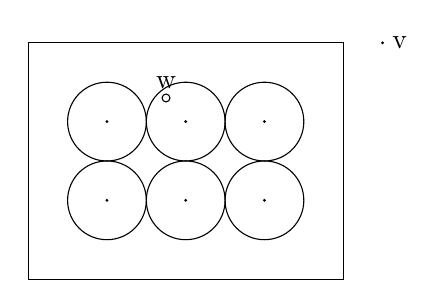
\begin{tikzpicture}
\draw (0,0) rectangle (4,3);

\draw (1,1) circle [radius=0.01]; \draw (1,1) circle [radius=0.5];
\draw (2,1) circle [radius=0.01]; \draw (2,1) circle [radius=0.5];
\draw (3,1) circle [radius=0.01]; \draw (3,1) circle [radius=0.5];

\draw (1,2) circle [radius=0.01]; \draw (1,2) circle [radius=0.5];
\draw (2,2) circle [radius=0.01]; \draw (2,2) circle [radius=0.5];
\draw (3,2) circle [radius=0.01]; \draw (3,2) circle [radius=0.5];

\node [above] at (1.75,2.3) {w}; \draw (1.75,2.3) circle [radius=0.05];
\node [right] at (4.5,3) {v}; \draw (4.5,3) circle [radius=0.01];

\end{tikzpicture}alle Wörter

\subparagraph{Definition}
Für Wörter $v,w \in \{ 0,1\}^n$ ist der Hamming-Abstand $d(v,w)$ die Anzahl Stellen, in denen sich $v,w$ unterscheiden.\\
Der Minimal-Abstand eines Codes $C$ ist $\min{\{d(v,w)|v,w\in C, v \neq w \}}$

\subparagraph{Satz}
\begin{enumerate}
\item Ein Code ist $k$-fehlererkennend genau dann wenn sein Minimalabstand mindestens $k+1$ ist.
\item Ein Code ist $k$-fehlerkorrigierend genau dann wenn sein Minimalabstand mindestens $2 k +1$ ist.
\end{enumerate}

Beweis:
\begin{enumerate}
\item "`$\Rightarrow$"' Sei $v$ ein Codewort und $w$ ein Wort mit $d(v,w) \leq k $. Wenn der Code 4-fehlererkennend ist, darf es demnach kein anderes Codewort $v'$ geben, welches einen Abstand $d(v,v') \leq k$ hat, da ansonsten $v'$ selbst kein Codewort mehr wäre, sondern ein Wort mit $k$ Fehlern. Daraus folgt, dass der Minimalabstand $d(v,v')$ des Codes mindestens $k+1$ ist.

"`$\Leftarrow$"' Für eine Codewort $v$ sei $s(v) = \{w | d(v,w) \leq k\}$. Aus $d(v,v') \geq k+1$ (Für alle Codewörter $v,v'$ für die gilt: $v \neq v'$):
\begin{itemize}
\item $\{v\} \cap s (v') = \varnothing$
\item $\{v'\} \cap s(v) = \varnothing$
\end{itemize}
(denn anonsten wäre der Abstand $\leq k$)\\
Jedes fehlerhafte Wort $w \in s(v)$, dass sich in höchstens $k$ Stellen von $v$ unterscheidet, kann somit erkannt werden.
\item ($\Rightarrow$) Seien $v$ ein Codewort und $w$ ein Wort mit $d(v,w) \leq k$. Wenn der Code $k$-fehlerkorrigierend ist, darf es nur ein Codewort $v$ mit $d(v,w) \leq k$ geben. Folglich muss $d(v',w) \geq k +1$ für alle Codewörter $v' \neq v$ gelten, woraus $d(v,v') \geq 2k +1$ folgt.\\
Daraus folgt, dass der Minimalabstand des Codes mindestens $2k+1$ ist.

($\Leftarrow$) Für ein Codewort $v$ sei $s(v) = \{ w | d(v,w) \leq k \}$. Aus $d(v,v') \geq 2k +1$ für Codewörter $v,v'$ mit $v \neq v'$ folgt $S(v) \wedge S(v') = \varnothing$ (denn angenommen $S(v) \wedge S(v') \neq \varnothing$, dann hätten $v,v'$ einen Abstand $\leq 2k$). Jedes $w \in S(v)$ lässt sich daher eindeutig zu $v$ decodieren.
\end{enumerate}

Beispiel: Der Minimalabstand des Parity-Check-Doe ist 2, da sich zwei Codewörter in mindestens $2$ Stellen unterscheiden. Folglich ist der Code 1-fehlererkennend und 0-fehlerkorrigierend.

Naiver Ansatz zur Fehlerkorrektur: Nachricht mehrfach senden.\\
Beispiel $0\rightarrow 000, 1 \rightarrow 111$\\
Der Code $\{000,111\}$ hat Minimalabstand 3 und ist daher 1-fehlerkorrigierend.\\
Nachteil: Platzverschwendung

Effizienter sind lineare Codes. Diese verwenden Matrix-Vektor-Operationen.\\
Beispiel: Mit $A=(\underbrace{1\dots 1}_{n})$ lässt sich der Parity-Check-Code beschreiben durch $\{ w \in \{0,1\}^n |Aw^T = 0\}$

\subparagraph{Definition} Ein Code heißt linear, wenn es eine Matrix $A$ gibt, so dass sich der Code darstellen lässt durch $\{ w | Aw^T = 0 \}$.\\
Folgerung:

\subparagraph{Satz} Ein binärer linearer Code $C$ ist ein Vektorraum über $\mathbb{Z}_2 (+,\cdot)$.\\
Beweis (Skizze):\\
Abgeschlossenheit der Vektoraddition: Zu zeigen: $w_1,w_2 \in C \Rightarrow w_1 + w_2 \in C$.\\
Aus $w_1,w_2 \in C$ folgt $A w_1^T = 0, A w_2^T = 0$ und daraus folgt $0= Aw_1^T + Aw_2^T =A(w_1 + w_2)^T$ und daraus folgt $w_1 + w_2 \in C$. Restliche Vektorraumaxiome folgen entsprechend.\\
Da ein linearer Code ein Vektorraum ist, besitzt er eine Basis.

\subparagraph{Definition} Sei $C$ ein linearer Code. Eine Matrix $G$, deren Zeilen eine Basis von $C$ bilden, heißt Generatormatrix.

Beispiel: Sei $G= \begin{pmatrix} 1 & 0 & 0 & 1 \\ 0 & 1 & 0 & 1\\ 0 & 0 & 1 & 1 \end{pmatrix}$. Die Zeilen von $G$ sind linearer unabhängig und es gilt $(b_1 b_2 b_3 ) \cdot  \begin{pmatrix} 1 & 0 & 0 & 1 \\ 0 & 1 & 0 & 1\\ 0 & 0 & 1 & 1 \end{pmatrix} = (b_1 \; b_2 \; b_3 \; (b_1 + b_2 + b_3) )$

Die Zeilen von $G$ bilden daher eine Basis für den Parity-Check-Code der Länge 4 und $G$ ist dessen Generatormatrix

Für den Minimalabstand eines linearen Code gilt:

\subparagraph{Satz} Sei $C$ ein linearer Code. Der Minimalabstand von $C$ ist $\min{\{d(c,0) | c \in C, c \neq 0\}}$.

Beweis: Seien $v,w \in C$ mit $v \neq w$. Da $C$ ein Vektorraum ist, gilt $v-w \in C$. Ferner unterscheidet sich $v-w$ von $0$ an genau den Stellen, an denen sich $v,w$ unterscheiden. Daraus folgt $d(v,w) = d(v-w,0)$ und damit $\min{\{ d(v,w) | v,w \in C, v \neq w \}} = \min{\{ d(c,0) | c \in C, c \neq 0\}}$.

Idee zur Konstruktion fehlerkorrigierender Codes: Mehrere Prüfsummen einfügen.

Beispiel $G= \begin{pmatrix}
1 & 0 & 0 & 1 & 1 & 0\\
0 & 1 & 0 & 1 & 0 & 1\\
0 & 0 & 1 & 0 & 1 & 1 \end{pmatrix}$.
Der erzeugte Code ist $C=\{ bG | b \in \{0,1\}^3 \}$ und $(b_1 b_2 b_3) \cdot G = (\underbrace{b_1 \; b_2 \; b_3}_{\text{Nachrichtenbits}} \underbrace{(b_1+b_2) \; (b_1+b_3) \;  (b_2+b_3)}_{\text{Prüfbits}})$.\\
Der erzeugte Code besteht aus 3 Nachrichtenbits und 3 Prüfbits. Der Minimalabstand ist 3, daher ist der Code 1-fehlerkorrigierend.







\end{document}